% everything defined here and before the `\begin` is called the preamble
% in here we define the document type, the language, the packages used, and some others
% this is basically a class and it controlls the look of thedocument
\documentclass[12pt, letterpaper]{article}
\usepackage[utf8]{inputenc}

% I'm literally just using this for centering the title page
% because I switched from report to article as my document class
% made the title and introduction on the same page
\usepackage{titling}
\renewcommand\maketitlehooka{\null\mbox{}\vfill}
\renewcommand\maketitlehookd{\vfill\null}

\usepackage[hidelinks]{hyperref}
\newcommand*{\email}[1]{\href{mailto:jhicks18@georgefox.edu}{\nolinkurl{jhicks18@georgefox.edu}} } 

% for IEEE format and bibliography
\usepackage[numbers]{natbib}
\bibliographystyle{IEEEtranN}

% for images
\usepackage{graphicx}
\graphicspath{ {./Images/} }

% for code blocks
\usepackage{listings}
\usepackage{color}

% defines the clor for significant code keywords
\definecolor{dkgreen}{rgb}{0,0.6,0}
\definecolor{gray}{rgb}{0.5,0.5,0.5}
\definecolor{mauve}{rgb}{0.58,0,.82}

% makes the code blocks look pretty :)
\lstset{frame=tb,
language=Scala,
aboveskip=3mm,
belowskip=3mm,
showstringspaces=false,
columns=flexible,
basicstyle={\small\ttfamily},
numbers=none,
numberstyle=\tiny\color{gray},
keywordstyle=\color{blue},
commentstyle=\color{dkgreen},
stringstyle=\color{mauve},
breaklines=true,
breakatwhitespace=true,
tabsize=3,
morecomment=[s]{\{- }{-\}},
morecomment=[l]{--}
}

% lets me include tabs if I want to :)
\newcommand\tab[1][1cm]{\hspace*{#1}} 

\title{A Brief Overview of Orc}
\author{Joshua Hicks}
\date{April 2021}

\begin{document}

\begin{titlingpage}
  \maketitle
\end{titlingpage}
\tableofcontents
\newpage
\section{Introduction}

Orchestration, better known as Orc, is a structured concurrent programming language that was developed by a team at the University of Texas in Austin, led by Jayadev Misra.  The project began in an attempt to solve their issues with other programming languages and their lack of convenient and well integrated concurrency primitives.  With the internet becoming such an important form of communication with people and machines around the world, their dream is to utilize the internet into a sort of 'global computer' where all services and data are available to all users at any time\cite{Cook2008}.  The team at UT Austin originally presented a solution with process calculus but it soon spiraled into a full programming language\cite{Kitchin2009}

Current programming languages rely on time-outs and interrupts which result in difficult and more error prone programs and while there are theoretical models in the space of concurrency which focus on expressive power and simplicity, they do not provide enough high-level constructs to be convenient in a developer's workflow. Therefore with this issue in mind UT Austin developed a theory called Orc where their guiding philosophy was to design a viable language that allows for structuring a program in a hierarchical manner and permit interactions among various subsystems in a controlled fashion\cite{Cook2008}.

\section{Syntactic and Semantic Features}
In Orc, we have two fundamental concepts wherein the magic of this language shines through: sites and combinators.  

\subsection{Sites}

Sites are similar to a method, subroutine, or function call in other programming languages.  What's significant here is that a site call might publish useful values, a signal, halt and publish nothing, or just wait indefinitely.  Some significant sites with Orc include:
\begin{lstlisting}
  Println("Hi") -- print out Hi to the console then publish a signal
  Random(10) -- publish a random integer from 0-9
  Browse("google.com") -- opens a browser window to google.com
\end{lstlisting}
While these are important sites to use within this language, Orc also takes some inspiration from Smalltalk where even the most basic operations are considered sites as well.  For instance \texttt{2 + 3} is just another way of writing the site call \texttt{(+)(2, 3)}\cite{Cook2008}.

\subsubsection{Literal Values}

Although sites are indeed important to this language and have many noteworthy mentions, the four literal values play a significant role for most, if not all, programs.  While other languages will have \texttt{Boolean}'s and \texttt{String}'s, Orc also uses \texttt{Number} which are a more abstracted version of floats and integers and the more interesting \texttt{signal} - a 'unitary' data value.  This is a very commonly used literal, yet it contains no information, rather it can be used to notify when a process or site is finished, or to ping another site to do something\cite{UserGuide}, such as below: 

\begin{lstlisting}
  def metronome() = signal | Rwait(1000) >> metronome()
\end{lstlisting}

This shows a recursive call to \texttt{Metronome} which will publish a \texttt{signal} every second, indefinitely.

\subsubsection{Type Inference}
Orc behaves, by default, as an untyped language however there is an optional static typechecker built in.  This can be enabled as a command line switch, or in Eclipse (if people even use that anymore...).  The type checker itself guarantees that no type errors will occur when ran.  This is a handy tool when dealing with some fairly clunky \texttt{read()} calls that will be touched upon later.

While type inferencing is a powerful feature with writability and readability in mind, there is still the option to add type information via the \texttt{::} symbol, which is very similar to Java and Scala.

\begin{lstlisting}
  {- Orc -}
  def square(x :: integer) = x * x

  /* Scala */
  def circleArea(x: int) x * x

  /* Java */
  public int circleArea(int x) { return x * x; }
\end{lstlisting}

Chaining these type hints in a multi clause function can become cumbersome and so Orc has added signatures where you can add an extra declaration instead of inline:

\begin{lstlisting}
  def sum(List[Number]) :: Number  {- a signature for 'sum' -}
  def sum([]) = 0
  def sum(h:t) = h + sum(t)
\end{lstlisting}

\subsubsection{Abstract Data Types}

Abstract data types are an interesting part of this language as datatypes are defined using the \texttt{type} declaration.  For instance, we could initialize a \texttt{Tree} as:
\begin{lstlisting}
  type Tree = Node(_,_,_)| Empty()
\end{lstlisting}
This declares two new sites called \texttt{Node} and \texttt{Empty}.  So as an example of usage we could build a \texttt{Tree} like so:
\begin{lstlisting}
  type Tree = Node(_,_,_) | Empty()
  {- Build up a small binary tree -}
  val l = Node(Empty(), 0, Empty())
  val r = Node(Empty(), 2, Empty())
  val t = Node(l, 1, r)
\end{lstlisting}
In this example we create a small binary tree where we store nodes in \texttt{l r} and \texttt{t}.

\subsubsection{Basic Flow of Control}

Flow of control in Orc is slightly unique in its implementation, as everything that is a seemingly significant part of this language is a site, so too are parts of the flow of control.   While there is the expression \texttt{if then else} where we can define the conditional expression between the \texttt{if} and \texttt{then} followed by the functions to execute, there is a more fascinating keyword we can use for comparisons that do not require an \texttt{else} clause.  \texttt{Ift} and \texttt{Iff} are sites that will publish a signal if the conditional expression is either true if false respectively.  This can be used in conjunction with combinators to make some very interesting operations.

\begin{lstlisting}
  -- Publishes: "Always publishes"
  Ift(false) >> "Never publishes"
| Iff(false) >> "Always publishes"
\end{lstlisting}

\subsection{Combinators}

Speaking of combinators, this is bread and butter of Orc where we can see its 'orchestration' ring through.  There are four types that we can use: parallel, sequential, pruning, and otherwise.  Each of these cominators forms and expression from two other component expressions and specifically capture a different aspect of concurrency\cite{UserGuide}.

\subsubsection{Parallel}

The parallel combinator is called with the \texttt{|} symbol and has the second highest precedence level out of the combinators.  We can use this combinator to join two different expressions in parallel.  For instance, we can call:

\begin{lstlisting}
  {- Publish 1 and 2 in parallel -}
  1 | 1 + 1
\end{lstlisting}

This will output \texttt{1} and \texttt{2} in parallel, such that which one gets published first is permutable.

\subsubsection{Sequential}

The sequential combinator has the highest precedence between these four operators and has a special relationship with \texttt{val}.  Syntactically, we use \texttt{>>} to execute and chain published values.  For instance \texttt{F >x> G} will result in any published value from \texttt{F} to be bound to \texttt{x} and whatever \texttt{G} publishes, mind you in parallel to \texttt{F}, will be published for the entire expression.

The two other uses of the sequential combinator include putting a pattern between the \texttt{>P>} where any published value from the left side is first filtered and then executes the right, and just the basic \texttt{>>} where there is an implied \texttt{\_} between the two such that every publication on the left will match the combinator pattern, therefore causing an execution of the right hand side for every individual publication of the left side\cite{UserGuide}.

This is special to variable bindings as instead of relying on the \texttt{val} and \texttt{let} keywords for declaration, you can simply bind between expressions.

\begin{lstlisting}
  {- Publish 1 and 2 in parallel -}
  (0 | 1) >n> n+1
\end{lstlisting}
This will output \texttt{1} then \texttt{2}.
\subsubsection{Pruning}

Although similar to the sequential combinator, we can use the pruning combinator to publish the right hand side as the result of the whole expression.  \texttt{F <x< G} will start by executing both \texttt{F} and \texttt{G} in parallel, but whenever \texttt{F} publishes a value, that value will be published for the entire execution.  When \texttt{G} publishes its first value, it will bind itself to \texttt{x} in \texttt{F} and then kill any more execution of \texttt{G}.  While waiting for \texttt{x} to be bound, \texttt{F} will simply be blocked until we have a published value from \texttt{G}.  This can potentially result in a inifitely long block state if \texttt{G} doesn't publish a value\cite{UserGuide}.

Similarly to the sequential combinator again, you can also put either a pattern or an implied \texttt{\_} between the \texttt{<<}.

\subsubsection{Otherwise}

Finally we have the otherwise combinator which is syntactically defined as \texttt{;}.  In a usecase such as \texttt{F ; G}, if \texttt{F} doesn't publish a value, then \texttt{G} will execute.  If not, then \texttt{G} will simply be ignored.  This has the lowset precedence level out of all the combinators.

\subsection{Combinator Application }  % @TODO this is a goofyass name, fix it 
As brought up in the abstract data section, we can take the defined \texttt{Tree} and \texttt{Node}s and extract ther contents with the pruning and parallel combinators in a manner such as:

\begin{lstlisting}
  {- And then match it to extract its contents -}
  t >Node(l,j,r)>
  r >Node(_,i,_)
  l >Node(_,k,_)>
  ( i | j | k )
\end{lstlisting}

This assigns \texttt{i}, \texttt{j}, and \texttt{k} to the published value from \texttt{t}, \texttt{r} and \texttt{l} such that calling \texttt{(i | j | k)} will publish \texttt{0 1 2} (where each value is placed on a separate line).

\subsubsection{Immutability}

Orc is a language which uses immutable variables and contains no assignment operators.  This doesn't seem to be an issue until you need to reassign a value, or want to define a variable before use.  Normally one would use the \texttt{val} keyword to create a variable, and in there perhaps assign a value from multiple site calls.  But consider this: in the Grammar program we needed to develop, a potential solution is using a \texttt{currentSymbol}.  This could be done with a clever use of recursion and parameter passing, but a simpler method would be to assign the value a \texttt{Ref()}.

Orc gives us two different mutable references to work with: \texttt{Cell()} and \texttt{Ref()}.  \texttt{Cell()} is a value that we can initialize before use, but only assign to once, while \texttt{Ref()} lets you assign values to it as many times as needed:

\begin{lstlisting}
  {- This will print out 0 then 2 -}
  val r = Ref(0)
  Println(r?) >>
  r := 2 >>
  Println(r?) >>
  stop
\end{lstlisting}

Interestingly this brings us to two more calls that can be summed up as 'syntactic sugar' which are the \texttt{read()} and \texttt{write()} calls.  In the code snippet above you could rewrite \texttt{r?} to \texttt{r.read()} and \texttt{r := 2} to \texttt{r.write(2)}.  The \texttt{?} operator is at the same precedence as \texttt{.} so you can chain then similar to how C uses the \texttt{*} with the only caveat being Orc using postfix instead of a prefix notation.

\section{Development Environment}

After this fairly general overview of Orc the main question is how to develop with it.  On the Orc homepage there are three options to choose from.  The first and very convenient one is to use their online development site where you can put in code snippets and check for their outputs.  While this is not nearly as powerful as developing on a personal device, especially with multiple assignments requiring the use of reading files outside of the program itself, it is still very nice to use when trying to debug potential syntactic issues.

Secondly there is an Eclipse extension that you can download from the Eclipse plugin store which will give you syntax highlighting and a built in compiler.  Unfortunately this language is very slow and any use from an ide such as autocomplete are not even supported resulting in Eclipse being slightly behind the other options, especially considering the fact that it is Eclipse.

Finally, there is an optional \texttt{.jar} file to download where you can run your code off the command line.

\section{Synopsis}

Overall Orchestration has many unique features that lend to an interesting language to dig through.  Unfortunately there are some areas to improve before it would feel ready to be adopted on a larger scale, but after working with this language throughout the semester some thoughts do stick out.

\subsection{Writability}

As an important factor for any language, writability can influence the choice between using the language or not.  Orc handles this section in dissapointingly neutral way, as orthogonally the language is impressive.  There are four distinct combinators and four literals that are all implemented orthogonally.  The main issue comes from sites, as while they are very powerful and lead to some very convenient uses, the lack of documentation make many potentially powerful operations unknown to the user, and the lack of detail makes it hard to take advantage of some of the best parts of this language.

\subsection{Readability}

When the writability works for Orc, it does it well.  Although the concise nature of this language does result in some code that might take a bit to dig through, the overall syntax of this language does a good job at making reading easier to understand.  Although in many official examples provided by the Orc development team have very unreadable variable names and little to no comments, if a developer chose to write good code with a standard naming convention it would be fairly natural to read.

\subsection{Personal Experience}

Orc is an interesting language that attempts to solve a fairly specific issue.  Unfortunately, with regards to the programming assignments required for this project, it was difficult to utilize the strengths of this language.  The documentation was very difficult to deal with as some sections in the offered wiki had multiple \texttt{TODO}'s that dated back to 2016, and trying to even figure out the supported methods of built in data structures were headache inducing.  Running the programs were very slow as 'futzing' around with the syntax and running the program multiple times with minimal changes really disrupted the workflow.  The command line was the best option for personal use, and while development consisted of using \texttt{vim} and a custom made \texttt{orc.vim} syntax file, having to deal with the long wait times became jarring.  Using the online development site was helpful to an extent but its limitations soon became apparent.

\begin{figure}[b]
  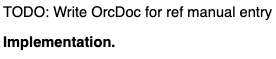
\includegraphics{documentation.png}
  \caption{A lack of documentation, or none at all can become frustrating when trying to learn a language.}
\end{figure}

\newpage
\bibliography{bibliography.bib}

\newpage

\section*{Programs}

\subsection*{n!}
\begin{lstlisting}
{-
 - Specified Implementation Details:
 -
 - Write a factorial program (preferably recursive) that accepts
 - a single integer n as input and outputs n!.
 - Input can be passed to the program as a command-line parameter
 - (preferred) or read from the keyboard.
 -
 - Note: if your language provides some sort of factorial function
 - or operation, write your own here to demonstrate how to write
 - (recursive) functions.
 -
 - ---
 -
 - Implementation Details:
 -
 - Prompt takes in the value
 - by surrounding the >> operator with the assignment to 'Number,'
 - I can pass in whatever is read from the Prompt via that value.
 -
 - Read(number) will convert whatever is inside to whatever
 - value it can infer, in this case it should be an int.
 -
 - To be more specific I could define the parameters
 - and return types in this manner
 -
 - def factorial(Number) :: Number
-}
def factorial(n) = if (n <= 1) then 1 else n * factorial(n - 1)

Prompt("What do you want to find the factorial of? ")
>number>
factorial(Read(number))
\end{lstlisting}

\subsection*{Output}
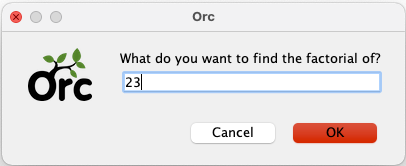
\includegraphics{n!-output.png}
Returns in the console: \texttt{25852016738884976640000}

\newpage

\subsection*{Structured Information Sorter}

\begin{lstlisting}
{-
 - Specified Implementation Details:
 - 
 - Write a program that keeps track of information about Persons.
 - A Person has a character string attribute called name and an
 - integer attribute called age.  If your language permits,
 - you should create an abstract data type for this kind of
 - information.  If your language does not have a mechanism
 - for building abstract datatypes such as a record, struct, 
 - class, etc., improvise.
 -
 - Your program should read from this data file of comma-delimited
 - name/age pairs and populate your program with a
 - collection (or array) of Persons.  Your program should
 - then sort the set by name, output the name of each 
 - Person in sorted order, and output the average age of
 - all the Persons.
 -
 - Note: if you find working with my datafile to be too difficult
 - you may either modify the structure (but not the order) of the
 - datafile or hard-code the data into your program
 - (while preserving the initial order of the data)
 - but you must jusitify your inability to perform I/O on the
 - existing datafile in your report.
 -
 - ---
 -
 - Implementation Details:
 -
 -}

{-
 - This sets up the .dat file and various imports needed to
 - read the Person.dat file
-}
val fileName = "Person.dat"
import class File = "java.io.File"
import class FileReader = "java.io.FileReader"
import class BufferedReader = "java.io.BufferedReader"
val file = File(fileName)
val reader = BufferedReader(FileReader(file))

{-
 - a Person site which holds a name and age.
 - I can use the `age :: Number` here to
 - give a type hint for the parameter,
 - so when I pass in a string of age, it will automatically convert
 - it to the proper data type
 -
 - on a side note, it is sometimes a little janky with type hints
 - so I specified `Read(age)` to make sure the age is
 - converted to a number
 -}
def class Person(name, age:: Number) =
    def getName() = name
    def getAge() = Read(age)
    stop

-- Reads the next line in the reader and converts it into a
-- Person site 
def getPerson() =
    val line = arrayToList(reader.readLine().split(","))
    Person(index(line, 0), index(line, 1)) 

-- recursively fills the provided array with Person sites
def initializePersonArray(index, array) =
    if (index <: 7) then array(index) := getPerson() >> initializePersonArray(index+1, array)
    else array 

-- grabs the indexed value of the array, and gets the average.
-- I recognize that this could be done with a lambda but
-- I'm having some issues figuring that out
def ageAverage(index, array, average) =
    if (index <: 7) then ageAverage(index+1, array, average+array(index)?.getAge())
    else average / index

val personArray = initializePersonArray(0, Array(7))
val nameArray = Array(7)

for(0, nameArray.length?) >i>
nameArray(i) := personArray(i)?.getName() >>
stop
;

sort(arrayToList(nameArray)) | "Average age: " + ageAverage(0, personArray, 0)

\end{lstlisting}

\subsection*{Output*}

\begin{lstlisting}
  "Average age: 35"
  ["Doe", "Flintstone", "Hansen", "Jones", "Schlablotnik", "Smith", "Smith"]
\end{lstlisting}

* Note that when using the parallel combinator the output is permutable.

\newpage

\subsection*{Random Text Generator}

\begin{lstlisting}
  {-
 - Re-implement the Random Text Generator program that
 - is assigned in approximately the 4th week of the course
 - using your programming language.
 -
 - Unfortunately this program took too long and is currently
 - unfinished...
 -}

val START_TOKEN = "{"
val END_TOKEN = "}"
val BODY_END = ";"

-- sets up the buffered reader 
val fileName = "pilot-episode.g"
import class File = "java.io.File"
import class FileReader = "java.io.FileReader"
import class BufferedReader = "java.io.BufferedReader"
val file = File(fileName)
val reader = BufferedReader(FileReader(file))

val startSymbol = Ref(null)

-- it's a dictionary with k: symbol v: list<symbol>
val symbolTable = Dictionary()
val symbolList = Ref([])

val leftHandSideSymbol = Ref(null)
val currentSymbol = Ref(null)
val readingAProduction = Ref(false)
val readingBodies = Ref(false)







def class Symbol(token :: String) =
    
    def getSymbol() = token
    def is(otherToken) = if (token?.equals(otherToken)) then true else false

    stop


def checkIfBody()  =
    val notAToken = Ref(true)
    -- If we're not yet reading a production check to see if
    -- the current symbol is the production start token
    if (readingAProduction? = false) then
        readingAProduction := currentSymbol.is(START_TOKEN) >>
        notAToken := false
    -- Otherwise see if the symbol is the production stop token
    -- If so, set the flag to indicate that we've hit the
    -- end of a production.  Otherwise we've got the head or
    -- body of a production
    else (Ift (currentSymbol?.is(END_TOKEN)) >>
        readingAProduction := false >>
        readingBodies := false >>
        notAToken := false) 
    ;notAToken?

def checkIfProduction() =
    val isProduction = Ref(false)
    -- there is the Iff operator that I could use instead of 
    -- readingBodies = false but this was sleeker to use
    Ift (readingBodies? = false) >> 
        isProduction := true >>
        leftHandSideSymbol := Symbol(currentSymbol) >>
        symbolTable.leftHandSideSymbol := [] >>
        readingBodies := true >>
        -- if this is the first left hand side we've seen
        -- then it's also the start symbol for the grammar
        Ift (startSymbol = null) >> startSymbol := leftHandSideSymbol
    ;isProduction?


-- Otherwise we're in the body of the production
def productionBody() =
    -- If the symbol is the end symbol, then we;re done reading a
    -- particular production body
    if (currentSymbol.is(BODY_END) then
        symbolTable.leftHandSideSymbol := symbolTable.leftHandSideSymbol?:symbolList
        symbolList := []
    -- Otherwise not at the end, add this symbol for the next
    -- production body we encounter
    else
        -- If the symbol is the literal string "\n" we'll turn that
        -- into an actual newline, otherwise just add the
        -- symbol to the list
        if (currentSymbol.is("\n") then symbolList := symbolList:Symbol("\n")
        else symbolList := symbolList:Symbol(currentSymbol)


def loopThroughFile(readingAProduction) =
    currentSymbol := reader.readLine()

    -- Otherwise we must be reading a production
    -- so this is the bead or bodies of a production
    Iff (checkIfBody()) >> Iff(checkIfProduction()) >> productionBody()


-- loopThroughFile(readingAProduction :: Boolean)
loopThroughFile(false)
\end{lstlisting}

\vspace*{\fill}
If anyone would like the orc.vim syntax file feel free to email \email{jhicks18}

\end{document}
